\documentclass{ncc}
\usepackage[utf8]{inputenc}
\usepackage[russian]{babel}
\usepackage[T2A]{fontenc}
\usepackage{amssymb}
\usepackage{amsmath}
\usepackage{pscyr}
\usepackage{graphicx}
\usepackage{listings}
\usepackage[colorlinks,linkcolor=black,urlcolor=blue]{hyperref}

\lstloadlanguages{C++}
\lstset{
language=C++,
extendedchars=\true, %Чтобы русские буквы в комментариях были
keepspaces=true,
inputencoding=utf8,
breaklines,
columns=fullflexible,
flexiblecolumns,
numbers=left,
numberstyle={\footnotesize},
commentstyle=\it,
stringstyle=\bf,
belowcaptionskip=5pt }


\title{Знакомство с дзета-функцией Римана}

\begin{document}
\maketitle
\tableofcontents
\section{Закон Стефана-Больцмана}

Если вкратце, то интегральная плотность потока энергии теплового излучения определяется законом Стефана-Больцмана:
\[
    P = \sigma T^4,
\]
где \( \sigma \) -- эмпирически полученная постоянная Стефана-Больцмана.
Эту же формулу можно получить из квантовых соображений, откуда можно получить теоретическое значение этой постоянной:
\[
    \sigma = \frac{k^4}{4 c^2\hbar^3}\int\limits_0^\infty\frac{x^3}{e^x-1}\,dx.
\]

Рассмотрим внимательнее интеграл в правой части. Попробуем его взять, разложиив в ряд:

\[
    \int\limits_0^\infty\frac{x^3}{e^x-1}\,dx = \int\limits_0^\infty\frac{e^{-x}x^3}{1-e^{-x}}\,dx = \int\limits_0^\infty x^3 \sum\limits_{n=1}^\infty e^{-nx}\,dx.
\]

Меняя местами интегрирование и суммирование, получаем
\[
    \sum\limits_{n=1}^\infty \int\limits_0^\infty x^3  e^{-nx}\,dx = \sum\limits_{n=1}^\infty\frac{1}{n^4} \int\limits_0^\infty t^3  e^{-t}\,dt =
    \Gamma(4)\sum\limits_{n=1}^\infty\frac{1}{n^4}.
\]

Про гамма-функцию поговорим как-нибудь в другой раз, а вот на сумме остановимся подробнее. Для неё существует отдельное обозначение

\[
    \sum\limits_{n=1}^\infty\frac{1}{n^4} = \zeta(4).
\]

Эта функция носит название \emph{дзета-функции Римана}.

\section{Определение}
Дзета-функция Римана \( \zeta(n) \) определяется выражением
\[
    \zeta(n) = \sum\limits_{k=1}^\infty \frac{1}{k^n}
\]
Особый интерес представляет определение значений этой функции через математические константы вроде \(\pi\) и \(\mathrm{e}\).

Рассмотрим сначала
\[
    \zeta(1) = \sum\limits_{k=1}^\infty \frac{1}{k}.
\]
В правой части стоит гармонический ряд, который расходится. Поэтому можно считать, что \( \zeta(1) = \infty \). При \( k \le 1 \) ряд, вообще говоря, расходится. Но это не обязывает обращаться \( \zeta(n) \) в бесконечность. Например,
\[
    \zeta(0) = 1 + 1 + 1 + \ldots = -\frac{1}{2}.
\]
Для расчёта в точках, в которых ряд не сходится, используется аналитическое продолжение. Именно поэтому появляются такие «парадоксы».

\section{\( \zeta(2) \). Доказательство Эйлера}
Многочлен \( P_n(x) \), множество корней которого \( \{ x_i \} \) можно представить в виде
\[
    P_n(x) = A\prod\limits_{i=1}^n (x-x_i).
\]
Но что если мы возьмем функцию с бесконечным числом корней и попробуем разложить её в произведение? Одним из первых до этого додумался Эйлер и представил в таком виде синус:
\[
    \sin x = Ax(x-\pi)(x+\pi)(x-2\pi)(x+2\pi)\ldots
\]
Константа определяется при помощи предела
\[
    \lim_{x\to0} \frac{\sin x}{x} = 1,
\]
откуда
\[
    \sin{x} = x\left(1-\frac{x^2}{\pi^2}\right)\left(1-\frac{x^2}{2^2\pi^2}\right)\ldots
\]
Попробуем получить несколько первых членов ряда Маклорена, раскрывая произведения:
\[
    \sin{x} = x - \sum\limits_{n=1}^\infty\frac{1}{n^2}\frac{x^3}{\pi^2} + \sum\limits_{n=1}^\infty\sum\limits_{m=n+1}^\infty\frac{1}{n^2m^2}\frac{x^5}{\pi^4} \ldots
\]
Сравним с рядом Маклорена:
\[
    \sin x = x - \frac{x^3}{6} + \frac{x^5}{120} - \ldots
\]
откуда
\[
    \zeta(2) = \sum\limits_{n=1}^\infty\frac{1}{n^2} = \frac{\pi^2}{6}.
\]
Кстати, необязательно использвовать синус -- подойдет и косинус:
\[
    \cos x = \left(1 - \frac{4x^2}{\pi^2}\right)\left(1 - \frac{4x^2}{3^2\pi^2}\right)\ldots
\]
Отсюда,
\[
    \sum\limits_{k=1}^\infty \frac{1}{(2k-1)^2} = \frac{\pi^2}{8}.
\]
Заметим, что
\[
    \sum\limits_{k=1}^\infty \frac{1}{(2k-1)^2} = \sum\limits_{k=1}^\infty \frac{1}{k^2} - \sum\limits_{k=1}^\infty \frac{1}{(2k)^2} = \frac{3}{4}\zeta(2),
\]
откуда можно получить ответ.

Вообще говоря, бесконечные произведения, посроенные таким образом, не обязаны совпадать с функцией. Например, \( e^z - 1 \) имеет корни \( 2\pi n i \), однако, произведение 
\[
    z\left[1+\left(\frac{z}{2\pi}\right)^2\right]\left[1+\left(\frac{z}{2\cdot2\pi}\right)^2\right]\ldots
\]
является нечётной функцией, и представляет из себя разложение \( \mathrm{sh\,}(z/2) \).

Можно получить тот же результат при помощи ряда Фурье функции \( x^2 \)
\[
    x^2 = \frac{\pi^2}{3} + 4\sum\limits_{n=1}^\infty\frac{(-1)^n}{n^2}\cos nx,
\]
рассмотрев его значение в точке \( x = \pi \).

Есть и другие способы, например интегральное представление и связь с числами Бернулли, о которых ниже.

\section{\(\zeta(4)\). Интегральное представление}
Используя то же разложение Эйлера, можно получить значение \( \zeta(4) \). Для этого заметим, что
\[
    \left(\sum\limits_{n=1}^\infty\frac{1}{n^2}\right)^2 = \sum\limits_{n=1}^\infty\frac{1}{n^4} + 2\sum\limits_{n=1}^\infty\sum\limits_{m=n+1}^\infty\frac{1}{n^2m^2}.
\]
Второе слагаемое справа мы уже втречали выше. Подставляя его значение, получаем
\[
    \zeta(4) = \zeta(2)^2 - 2\frac{\pi^4}{120} = \frac{\pi^2}{90}.
\]

Этот результат можно получить и другими способами. Нетрудно убедиться, что
\[
    \sin(x)\sin(ix) = ix^2\left(1-\frac{x^4}{\pi^4}\right)\left(1-\frac{x^4}{2^4\pi^4}\right)\ldots
\]

Также можно использовать ряд Фурье функции \( x^4 \)
\[
    x^4 = \frac{\pi^4}{5} + \sum\limits_{n=1}^\infty\left(\frac{8\pi^2}{n^2}-\frac{48}{n^4}\right)(-1)^n\cos nx
\]
в точке \( x=\pi \).

В самом начале статьи нами было получено
\[
    \int\limits_0^\infty \frac{x^3\,dx}{e^x - 1} = \Gamma(4)\sum\limits_{n=1}^\infty\frac{1}{n^4}.
\]
Обобщая для произвольного \( n \), получаем интегральное представление:
\[
    \zeta(n) = \frac{1}{\Gamma(n)}\int\limits_0^\infty \frac{x^{n-1}\,dx}{e^x - 1}
\]

\section{Значения в других чётных точках}

\subsection{Через степени \(\zeta(2)\)}
Совершенно аналогично тому, как это было сделано для \( \zeta(4) \), можно получить выражение для любого \( \zeta(2m) \). Для начала получим \( \zeta(6) \), возводя \( \zeta(2) \) в куб:
\[
    \left(\sum\limits_{k=1}^\infty \frac{1}{k^2}\right)^3 = \sum\limits_{k=1}^\infty \frac{1}{k^{6}} + 3\sum\limits_{k=1}^\infty\sum\limits_{m\ne k} \frac{1}{k^{4}}\frac{1}{m^2} + 3!\sum\limits_{k=1}^\infty\sum\limits_{m>k}\sum\limits_{n>m}\frac{1}{k^2}\frac{1}{m^2}\frac{1}{n^2}
\]
Сумму во втором слагаемом можно найти из следующих соображений:
\[
    \zeta(2)\zeta(4) = \zeta(6) + \sum\limits_{k=1}^\infty\sum\limits_{m\ne k} \frac{1}{k^{4}}\frac{1}{m^2},
\]
а сумму из третьего слагаемого -- при помощи следующего члена ряда Маклорена:
\[
    \sum\limits_{k=1}^\infty\sum\limits_{m>k}\sum\limits_{n>m}\frac{1}{k^2}\frac{1}{m^2}\frac{1}{n^2} = \frac{\pi^6}{7!}.
\]
Собрав всё вместе, получим
\[
    \zeta(2)^3 = \zeta(6) + 3(\zeta(2)\zeta(4)-\zeta(6)) + \frac{3!\pi^6}{7!},
\]
откуда
\[
    \zeta(6) = \frac{\pi^6}{945}.
\]

Дальше становится всё сложнее и более громоздко, поэтому рассмотрим другие способы.

\pagebreak
\subsection{Вычисление интеграла}
Для вычисления интеграла воспользуемся интегрированием по контуру в комплексной области. Выберем контур следующим образом:

\begin{figure}[h]
    \center
    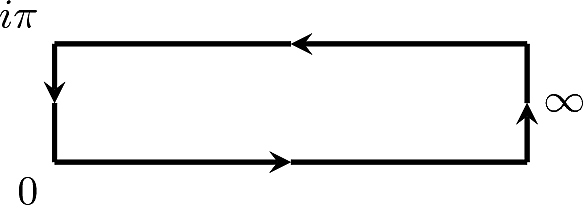
\includegraphics[width=.5\textwidth]{2015-12-13-riemann-zeta-contour.png}
\end{figure}

Тогда
\[
    \oint\limits_C \frac{z^{n-1}\,dz}{e^z-1} = \int\limits_0^\infty \frac{x^{n-1}\,dx}{e^x - 1}  - \int\limits_0^\infty \frac{(x+i\pi)^{n-1}\,dx}{-e^x - 1} - \int\limits_0^\pi \frac{i^ny^{n-1}\,dy}{e^{iy} - 1} = 0.
\]
Немного преобразуем:
\[
    \int\limits_0^\infty \frac{x^{n-1}\,dx}{e^x - 1}  + \sum\limits_{k=0}^{n-1}C_{n-1}^k(i\pi)^k\int\limits_0^\infty \frac{x^{n-1-k}\,dx}{e^x + 1} = i^n\int\limits_0^\pi \frac{(\cos y - 1 - i\sin y) y^{n-1}\,dy}{2(1-\cos y)}.
\]
Сведём второй интеграл в левой части к первому:
\[
    \int\limits_0^\infty \frac{x^{n-1}\,dx}{e^x + 1} =
    \int\limits_0^\infty \frac{x^{n-1}\,dx}{e^{x} - 1} -
    \int\limits_0^\infty \frac{2x^{n-1}\,dx}{e^{2x} - 1}=
    (1-2^{1-n})\int\limits_0^\infty \frac{x^{n-1}\,dx}{e^{x} - 1}.
\]
Обозначим \( I_n = \Gamma(n)\zeta(n) \). Получаем
\[
    I_n  + \sum\limits_{k=0}^{n-1}C_{n-1}^k(i\pi)^k(1-2^{1-n+k})I_{n-k} = -i^n\left(\int\limits_0^\pi \frac{y^{n-1}\,dy}{2} + \int\limits_0^\pi \frac{i y^{n-1}\sin y\,dy}{2(1-\cos y)}\right).
\]
Рассмотрим случай \( n = 2m \) и выделим действительную часть:
\[
    I_{2m}  + \sum\limits_{k=0}^{m-1}C_{2m-1}^{2k}(-1)^k\pi^{2k}(1-2^{1-2m+2k})I_{2(m-k)} = (-1)^{m+1}\frac{\pi^{2m}}{4m},
\]
откуда
\[
    \zeta(2m)  = \frac{(-1)^{m+1}\pi^{2m}}{4(1-2^{-2m})(2m)!} + \sum\limits_{k=1}^{m-1}\frac{(-1)^{k+1}\pi^{2k}}{(2k)!}\frac{2^{2m-1}-2^{2k}}{2^{2m}-1}\zeta(2m-2k).
\]
Посчитаем несколько значений:
\[
\begin{array}{l}
\zeta(2) = \frac{\pi^2}{4(1-1/4)\cdot 2} = \frac{\pi^2}{6},\
\zeta(4) = -\frac{\pi^4}{4(1-1/16)\cdot 24}+\frac{\pi^2}{2}\frac{8-4}{16-1}\frac{\pi^2}{6}= -\frac{\pi^4}{90}+\frac{4\pi^4}{180}=\frac{\pi^4}{90},\
\zeta(6) = \frac{\pi^6}{4(1-1/64)\cdot 720}+\frac{\pi^2}{2}\frac{32-4}{64-1}\frac{\pi^4}{90} - \frac{\pi^4}{24}\frac{32-16}{64-1}\frac{\pi^2}{6}= \frac{3\pi^6}{63\cdot 45} = \frac{\pi^6}{945}.
\end{array}
\]

Но всё-равно хочется более короткой и выразительной формулы. Для этого свяжем зета-функцию и числа Бернулли.

\section{Связь с числами Бернулли. Производящая функция}
Вернёмся к бесконечному произведению
\[
    \sin x = x\prod\limits_{n=1}^\infty\left(1-\frac{x^2}{n^2\pi^2}\right)
\]
Возьмём логарифм от обеих частей
\[
    \ln\sin x = \ln x + \sum\limits_{n=1}^\infty \ln\left(1-\frac{x^2}{n^2\pi^2}\right)
\]
и продифференцируем
\[
    \frac{\cos x}{\sin x} = \frac{1}{x} + \sum\limits_{n=1}^\infty \frac{-\frac{2 x}{\pi^2 n^2}}{1-\frac{x^2}{n^2\pi^2}},
\]
а потом домножим на \( x \) и немного преобразуем:
\[
     x\frac{\cos x}{\sin x} = ix + \frac{2ix}{e^{2ix}-1} = 1 -2\frac{x^2}{\pi^2 n^2}\sum\limits_{n=1}^\infty\sum\limits_{k=0}^\infty \frac{x^{2k}}{n^{2k}\pi^{2k}},
\]
В левой части мы видим производящую функцию чисел Бернулли:
\[
    \frac{2ix}{e^{2ix}-1} = 1 - \frac{1}{2}\cdot 2ix + \sum\limits_{k=1}^\infty B_{2k}\frac{(2ix)^{2k}}{(2k)!}.
\]
Пользуясь этим разложением и меняя порядок суммирования справа, получаем
\[
      \sum\limits_{k=1}^\infty B_{2k}\frac{(2ix)^{2k}}{(2k)!}= -2\sum\limits_{k=1}^\infty\sum\limits_{n=1}^\infty \frac{x^{2k}}{n^{2k}\pi^{2k}},
\]
\[
      \sum\limits_{k=1}^\infty \frac{(-1)^k2^{2k}B_{2k}}{(2k)!}x^{2k}= -2\sum\limits_{k=1}^\infty \frac{\zeta(2k)}{\pi^{2k}}x^{2k},
\]
откуда имеем
\[
    \zeta(2k) = \frac{(-1)^{k+1}}{2}\frac{(2\pi)^{2k}B_{2k}}{(2k)!}.
\]

Вернёмся к функции \( x\mathrm{ctg\,} x \):
\[
    x\mathrm{ctg\,} x = 1 - 2\sum\limits_{k=1}^\infty \frac{\zeta(2k)}{\pi^{2k}}x^{2k}.
\]
Отсюда нетрудно получить
\[
    -\frac{\pi x}{2}\mathrm{ctg\,}\pi x = -\frac{1}{2} + \sum\limits_{k=1}^\infty \zeta(2k)x^{2k}.
\]
Так как 
\[
    \zeta(0) = 1 + 1 + 1 + \ldots = -\frac{1}{2},
\]
то функция
\[
    G(x) = -\frac{\pi x}{2}\mathrm{ctg\,}\pi x = \sum\limits_{k=0}^\infty \zeta(2k)x^{2k}
\]
является производящей функцией для значений дзета-функции в чётных положительных точках.

\section{Продолжение следует}

Про значения в нечётных точках известно немногое, и у меня пока нет идей на их счёт. В следующей части будут аналитическое продолжение, функциональное уравнение дзета-функции, а также немножко про нули и гипотезу Римана.
\end{document}
